\chapter{Subjective Experiment}
\label{chap:subjective}
This chapter covers everything there is to know about why and how we conducted and designed our subjective experiments. First and foremost we will describe the steps we took, as well as the considerations we had to make in order to create well-thought-out surveys. Those sections are followed by an introduction to the three datasets provided by Mobai, as well as an in-depth description of our own dataset. 

\section{Conducting the Survey}
\label{sec:ConductingSurvey}
The main reason for arranging a subjective experiment, was to collect ground truth data that would determine whether the quality scores provided by the metrics were accurate. As mentioned in Section \ref{section:academic background}, our lack of experience indicated that an introduction to the topic was needed. The research about conducting a subjective survey made us realize the importance and difficulties with this task. There were several assessments to perform in terms of creating a comprehensive subjective survey.

 %what is ground truth data
 
\subsection*{Survey Scope}
A crucial factor in the making, was the survey's scope. It was important that the observer had a sufficient number of images to evaluate for the validation purposes of the ground truth data. However, it would not benefit each observer to have a giant workload. Too much facial image evaluation would cause for example eye fatigue and headache. These kind of disorders would affect the subjective scores negatively, resulting in the data to be invalid. 

Our solution included separating the experiment into three individual parts. Each session consisted of more or less 100 facial images for the observers to evaluate. Combined, 294 images made up the whole dataset. We thought the survey's scope was fine-tuned, especially in regard to the duration of completing the survey. We also specified to the observers in the survey instruction manual, described in Section \ref{sec:intromanual}, to take a break of minimum five minutes between each session to feel refreshed. The duration of the subjective experiment including breaks was estimated to take approximately 45 minutes. In our opinion, this was a reasonable time span in terms of making observers participate in the survey without making them bored. 

\begin{figure}[h]
    \centering
    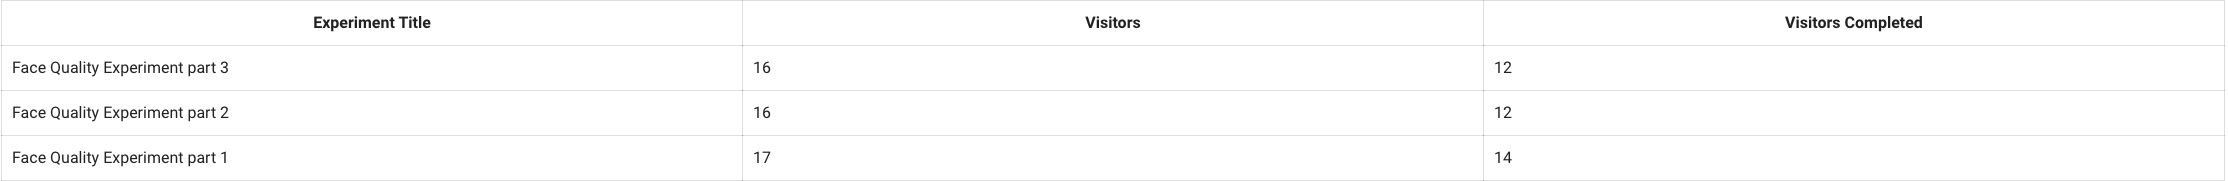
\includegraphics[scale = 0.2]{figures/three-sessions.png}
    \caption{Survey separated in three sessions}
    \label{fig:three-sessions}
\end{figure}

\subsection*{Displaying Images Randomly}
Early in the survey development process, we knew the ordering of the facial images would affect the total subjective scores at the end (kilde). On that account, we decided to display images in a random order to each observer. The primary reason for our choice was the elimination of bias data. Having the image sets shown in the same order for every participant would result in score biases, because observers are more attentive at the beginning of the experiment than towards the end. Having a unique question sequence for every observer would result in reliable subjective scores. Secondly, randomizing questions preserved every observer to give their honest opinion on the facial images, without sharing answers with other participants.

\subsection*{Judgment Methods}
A judgment scale was another key factor to take into account for the subjective survey. We needed to provide the observers with an easy scale to rate the facial images. Mobai suggested to rate the images on a scale from 1 to 100, because both metrics provided this output. We suppressed the proposal, with two main arguments: First, it would be extremely challenging for the observers to know the difference between close score ratings (e.g. an image with a score of 61 and an image with a score of 65). Second, the larger the judgment scale was, the more time consuming it would be to complete the survey. We felt that even rating facial images using a ten-point scale was too arduous. 

A way that made the subjective experiment more interesting for the users, was to vary in ratings methods. Initially we found this idea useful. In addition to using a category judgment, we discussed the option of using a rank order system in one of the sessions. The observers would rate images by drag-and-dropping them into different categories. The rank order system idea got terminated quickly. We had to preselect images of different quality for the observers to assess, resulting in bad data in terms of leading answers. Mixing different ranking methods would also boost the experiment duration due to multiple tasks the participants have to learn. 

Our final deployable survey consisted of a category judgment method while using a five-point scale. Here, one was poor, two was bad, three was fair, four was good and five was excellent. The reason for this scale system was in regard to the observers. Given 305 images to evaluate, it was easy for the participants to assess the facial images within a reasonable time slot and did not require extensive training. Another reason for using the category judgment method was to receive sufficient and easy-to-process data to correlate with the FIQMs.

\subsection*{Choice of Survey Software}
\label{subsection:choicesoftware}
A decision we thought would be easy, but ended up being challenging and time consuming was the choice of survey software. There were a bunch of opportunities for conducting the survey. However, we had to bare in mind the factors described above in our choice. One survey software we found interesting was Survey Monkey. The main reason we abstained from Survey Monkey was their demand of creating a yearly subscription to use the included functions as displaying questions in random order. We even asked for a four month subscription without luck. Another software we found appropriate was Survey Legend, a survey software perfectly suitable for images. It included many functions we needed, except enabling questions to be ordered randomly for each observer. Therefore, we unfortunately had to abort Survey Legend as well. 

After some inspiration and advice from our supervisor, we ended up arranging the subjective experiment in QuickEval - a survey software provided by NTNU. The software provided every functionality we needed such as category judgment and random order of questions. We produced three survey sessions easily by adding datasets to the application. QuickEval formatted each image in the center of the screen with a neutral dark grey background, but we had to make sure every image in the datasets were similar in size. Our psychometric experiment was available for everyone to participate, but specific employers at Mobai and NTNU were specially invited. This to get answers from experts in the field. QuickEval displayed statistics in the application gradually as people responded to the experiment. The statistics data was also downloadable as a CSV, HTML or Excel file. 
Using QuickEval as a survey handler ended up being a good choice because it was created by NTNU and we had a close relationship with the developers. When an issue occurred, we submitted that issue and communicated directly with a developer resulting in the issue to be fixed quickly. 

\section{Covid-19 Pandemic Implications}
Due to the ongoing Covid-19 pandemic, limitations with the subjective experiment occurred. We did not have the opportunity to create a controlled environment and invite the participants to complete the subjective experiment there. Ideally, such a controlled environment would be a well-lit room with good air quality, timed breaks between the sessions and a computer with specific screen settings for all participants to complete the experiment on. The Norwegian Colour and Visual Computing Laboratory in NTNU Gjøvik would be a complete environment that could be standardized according to International Commission of Illumination (CIE) publications, but unfortunately this was not achievable given the Covid restrictions. For that reason, all the participants completed the subjective experiments in an uncontrolled environment using their own computers with their custom screen resolution and lighting conditions. Factors such as the monitor brightness and color temperature and even the participants distance from the monitor as well as the illuminance of the room, matter. These custom settings are tiny factors that likely can alter the perception of the images in the survey and provide cognitive biased scores. The design of the survey was therefore important. QuickEval had an already built-in neutral and balanced gray background, which is considered by psychologists to not trigger any emotions. Since the participants performed the survey at different environments, not influencing the participants´s moods were important \cite{grayBackground}. 

We had no opportunity to control the length of the breaks between the sessions or if even breaks were held. However, in QuickEval we had the opportunity to review the observers' breaks by monitoring the timestamps between starting each session and the review showed that none of the sessions were taken right after each other.  

\section{Types of Participants}
As mentioned in \ref{subsection:choicesoftware}, the experiment was available for everyone to perform, but we invited a specific target group that works in this field. The types of participants are divided in two groups: experts and non-experts.

\subsection*{Experts}
The experts are the people who were specially invited to complete the survey. These observers work either for Mobai with facial recognition systems or at NTNU in the Faculty of Information Technology and Electronics. A point of having experts in the field doing the survey was to quality assure our creation since they to a larger degree can distinguish between quality issues. In addition to that, we were to compare the results between the two groups. 

\subsection*{Non-experts}
Non-experts were people with no experience in the biometric field. They were our friends and family of different ages and educations or people who arbitrary came across the experiment on the web. 

\section{Introduction Manual}
\label{sec:intromanual}
When conducting the subjective experiment and collecting the ground truth data, we wanted the subjective scores of the facial images to be similar. That meant all observers should give equal rating to an image. In order to manage this, we needed to create a uniform understanding for the observers on how they should perform the survey. Thus, a survey instruction manual was made. 

The first clarification we had to convey to the participants, was the meaning of face image quality. Both experts and non-experts would have different perceptions in terms of face image quality and we had to clarify all factors affecting face image quality - not only the resolution. 

The most clear and effective way to train the observers was to visualize examples of rated images like they would do in the survey. We created five example lineups with selfies of ourselves. Those facial images included most issues affecting the quality of an image. 

\begin{figure}[h]
    \centering
    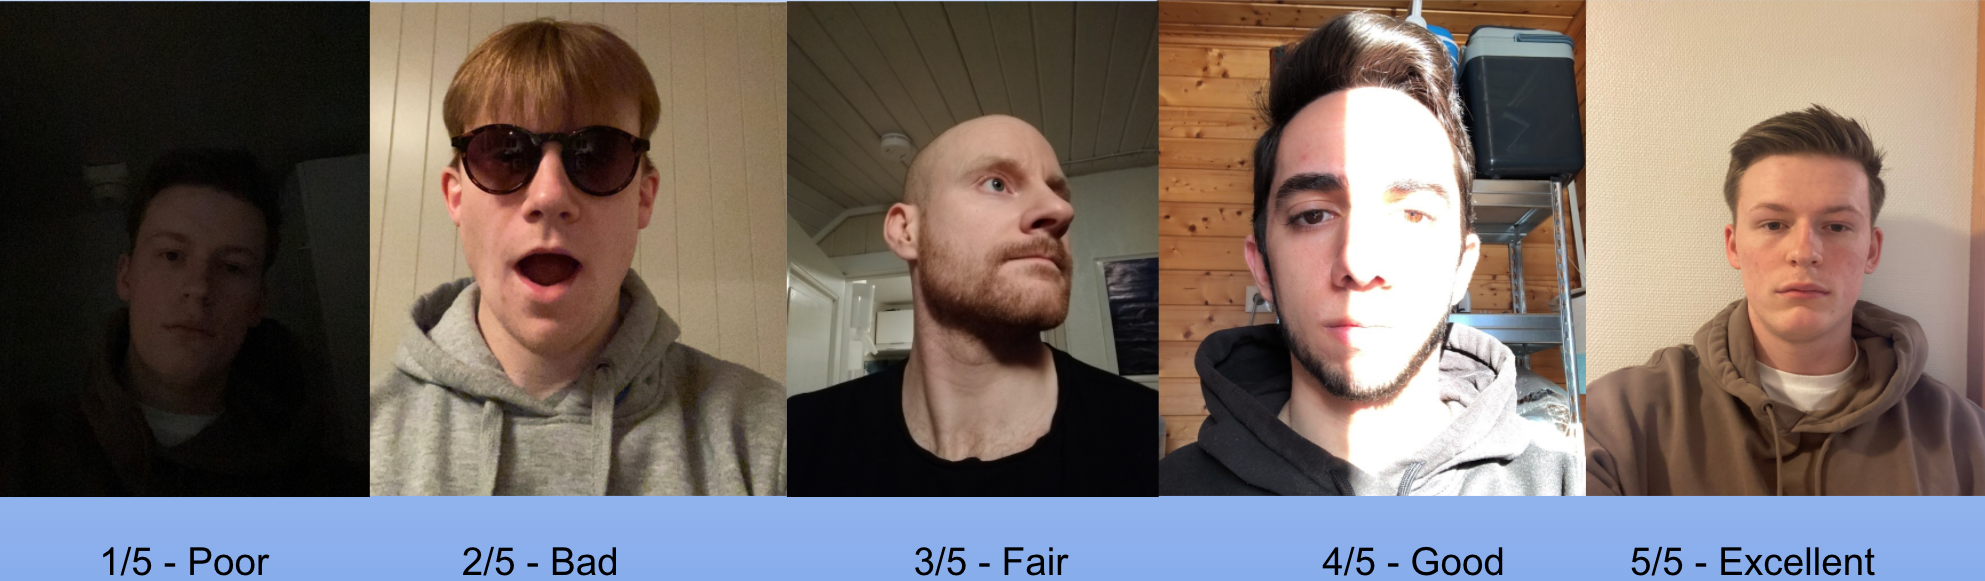
\includegraphics[scale = 0.23]{figures/Example-lineup.png}
    \caption{A lineup from the introduction manual}
    \label{fig:example-manual}
\end{figure}

The lineup images in Figure \ref{fig:example-manual} were a good guidance on how to rate the images. In the survey however, some participants found it harder to rate the survey images, because they included several image properties to take into account. 

\section{Datasets}
\label{sec:datasets}
The usage of facial images in the application and survey raised a lot of GDPR issues. It would strike against the rules if we photographed people on the streets or collected random images on the web without consent from the subjects. Mobai provided us with three approved datasets with different image attributes: \textbf{Combined passport alike} was a high resolution dataset which has a similarity to passport or id photos, hence the title. The set consisted of 98 facial images of people with different poses, facial expressions and lighting. All images were taken with a \textbf{NIKON D3100} with a dark blue or light grey background. The camera distance was equal in every photo and the camera lens was in an even height with the faces. 
\begin{figure}[h]
    \centering
    \subfloat[\centering]{{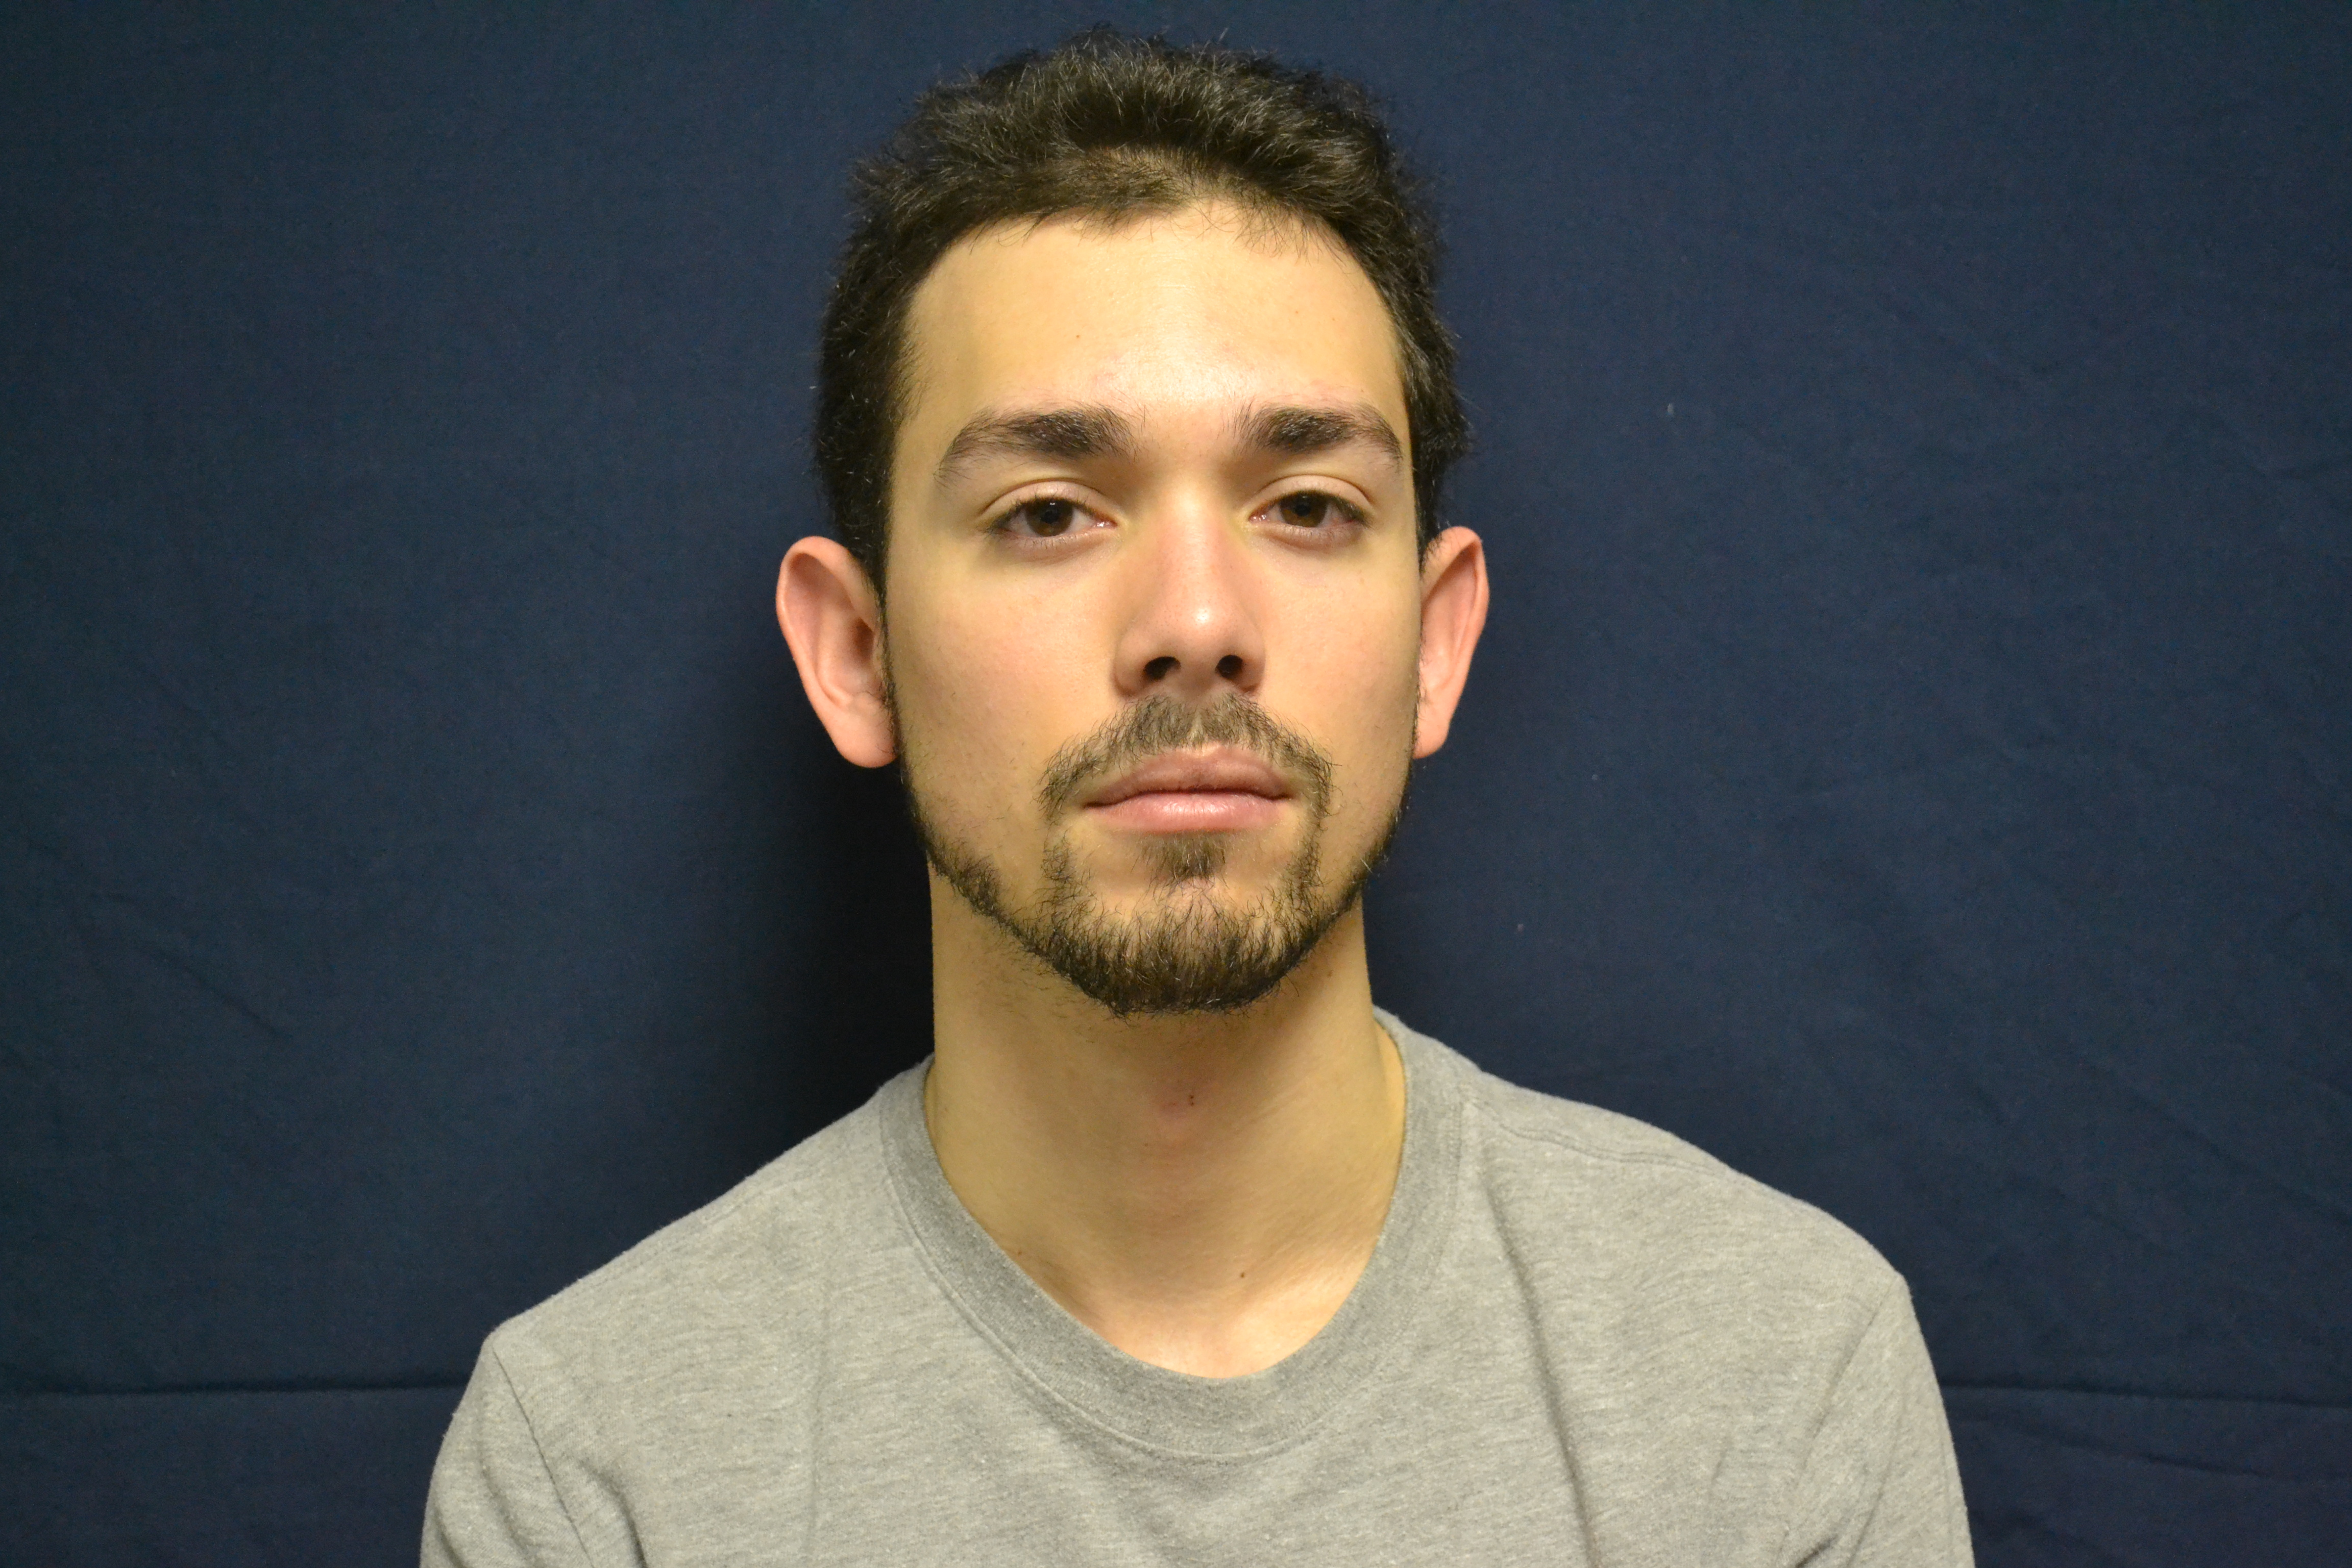
\includegraphics[width=5cm]{figures/0.jpg} }}
    \qquad
    \subfloat[\centering]{{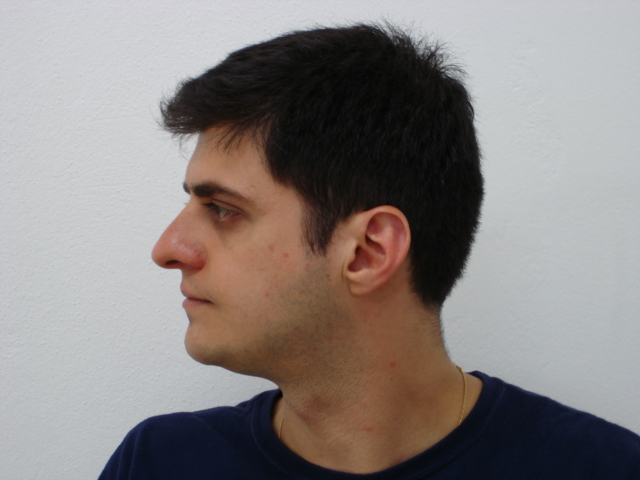
\includegraphics[width=5cm]{figures/50.jpg} }}
    \caption{Facial images from Combined passport alike}
    \label{fig:combined_passport_alike}
\end{figure}
\newpage
\noindent
\textbf{Capture from photo} was created by several employees at NTNU. All 70 images were selfies, taken with different phone cameras. Like Combined passport alike, the people had disparate poses and facial expression. However, in this dataset, the images were photographed in multiple locations on campus, which made the background and lightning vary considerably. Some of the images were captured from computer screens that would possibly affect the FIQM's evaluation scores. 

\begin{figure}[h]
    \centering
    \subfloat[\centering]{{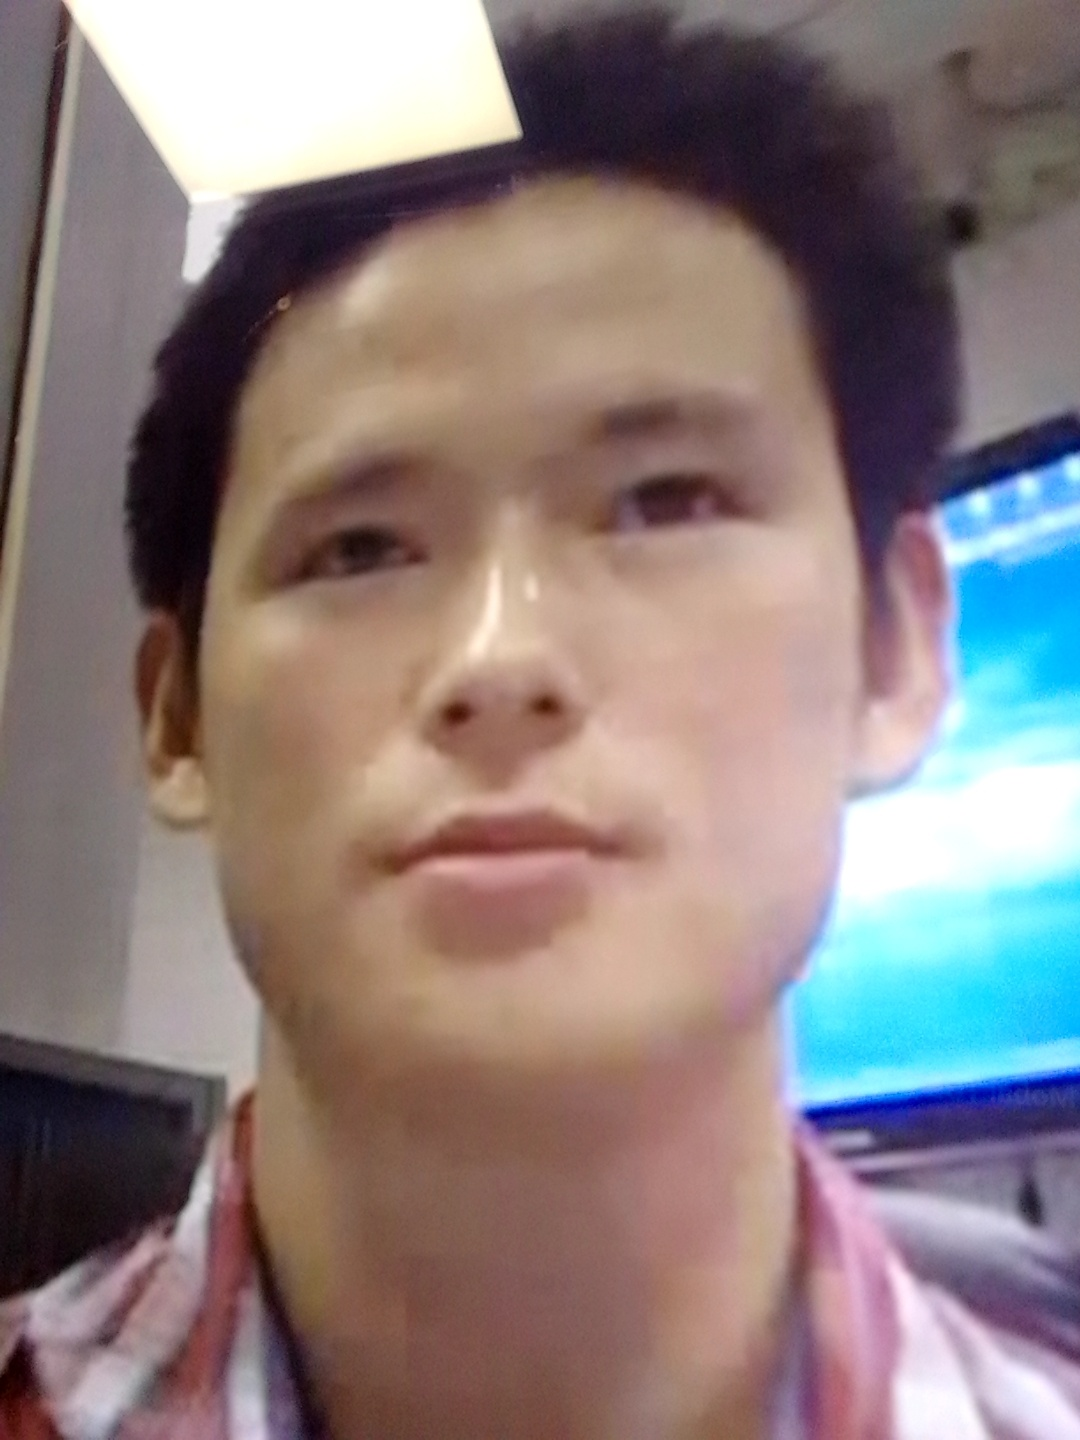
\includegraphics[width=4cm]{figures/1_0.89185.jpg} }}
    \qquad
    \subfloat[\centering]{{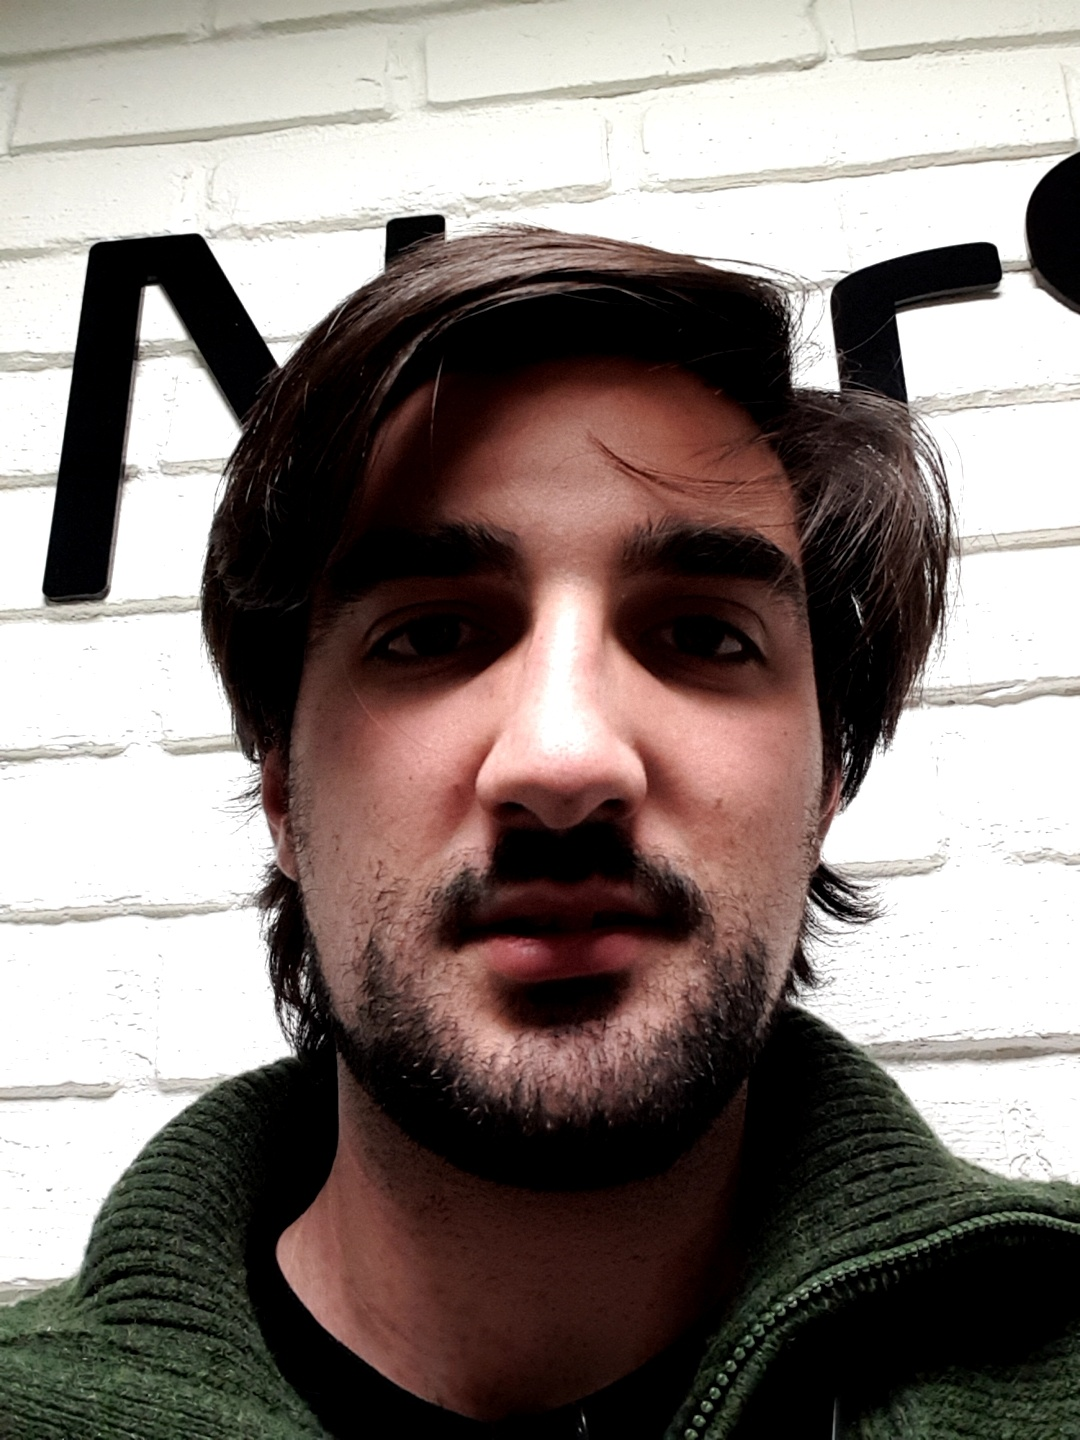
\includegraphics[width=4cm]{figures/3_0.74371.jpg} }}
    \caption{Facial images from Capture from photo}
    \label{fig:capture_from_photo}
\end{figure}
\noindent
The \textbf{Selfie dataset} was a set of 126 images accessible on the web. The images were selfies of different people at numerous locations: both indoors and outdoors. Given the selfies, the photos were taken with phone cameras and the camera to subject distance was short. 
\begin{figure}[h]
    \centering
    \subfloat[\centering]{{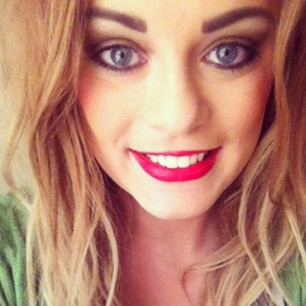
\includegraphics[width=4cm]{figures/10249165_693227110715964_1497214365_a.jpg} }}
    \qquad
    \subfloat[\centering]{{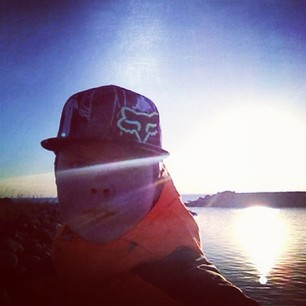
\includegraphics[width=4cm]{figures/10251439_436588196485138_396348425_a.jpg} }}
    \caption{Facial images from Selfie dataset}
    \label{fig:selfie_dataset}
\end{figure}
\noindent
The images within the three datasets were mixed up and used in the experiment sessions. We combined the images equally, meaning that one third of every dataset was included in each session. A mixture of image types prevented the observers of getting bored and evaluate badly due to monotonous types of facial images. 

\subsection{What went wrong?}
Despite conducting the survey in uncontrolled environments, the accomplishment of the subjective experiment was successful. There were gathered a reasonable number of participant relatively quick which resulted in having more time analyzing the data. Since it was our first time creating this kind of experiment, some experiment aspects were left out of the consideration that could be important. The main flaw with this experiment, was the lack of information about observes' characteristics, especially color blindness. Research show that colour vision deficiency (CVD) affects eight percent men and 0.5 percent women in the world \cite{colorblindness}. Given that 87 percent of the observers participating in our survey were men, there was a possibility that color blindness existed among the observers. People with a type of color blindness have the capability to discern colors to a lesser degree than people with a normal color vision. Therefore, this will affect the way they assess the facial images which is the reason why they are not contemplated as optimal observers \cite{Xphdthesis}. A good solution would be to test all participants with standardized color vision tests like an Ishihara test or a Cambridge color test.   

\subsection{Creating our own dataset}
\label{sec:ownData}
When working with machine learning and AI in context of face recognition, the probability of using one of the famous pre-curated \textbf{Labeled Faces in the Wild (LFW)} datasets is highly likely. Conditions such as poor lightning, extreme poses and face coverings are somewhat lacking in LFW and these are all important aspects for Mobai´s face recognition system. We saw the opportunity to contribute with a specialized dataset designed to fit Mobai´s needs which led to the proposal of a new dataset. Our initiative was positively received by Mobai.

The idea to collect a new dataset came about when the team was discussing flaws with the Selfie dataset. Mobai´s definition of face quality is, as mentioned in Section \ref{sec:setup}, originally based on ISO 29794-5 and ICAO Doc 9303 Part 3. Based on those definitions, one could argue that the images in the Selfie dataset did not fulfill the criteria. A significant part of the images in the selfie dataset are of faces that either are way off-centered, too zoomed in or a combination of both. We figured it could be valuable for Mobai to have a new dataset aligned with certain criteria they valued. 

\subsection*{Creation Process}
We had initially taken a few images of ourselves which were used for the instruction manual, illustrated in Figure \ref{fig:example-manual}, to the subjective experiment. These images were included in the dataset we started gathering. We came to the conclusion that each day, starting 1. Mars and ending 15. April, we would capture at least five selfies of ourselves every day. This would wind up to be at least 250 images of each member, which in the end equaled a dataset consisting of 1172 images. Our dataset is relatively large in size in comparison to the combined dataset used in our experiment. Some of the images are similar to the Combined passport alike dataset in regards to pose, but our dataset includes several varieties and specialized conditions which will be presented below. 

All the images were captured using both the front and back camera of our mobile phones. This lead to our dataset containing images of varying resolution, given that our phones were not of the same type. The phones used for the dataset collection were:
\begin{itemize}
    \item Apple iPhone 8 
    \item Apple iPhone 11 (2 units)
    \item Motorola Moto G5S Plus 
\end{itemize}
These had different camera specifications with the front cameras ranging from seven to 12 megapixels and the back cameras ranging from 12 to 13 megapixels. The change in image resolution was very minor which makes the differences barely noticeable and insignificant in regards to the face image quality.

\subsection*{Contents}
Our dataset was inspired by the three datasets mentioned in Section \ref{sec:datasets}, but was unique because elements like camera tilting and face masks were represented. During our image collection, we gathered examples of our faces with: 
%
\begin{itemize}
    \item Different lightning conditions.
    \item Different facial expressions and head poses.
    \item Different face and head coverings. 
    \item Different camera angles and camera tilts.
    \item Different backgrounds.
\end{itemize}
%
A crucial consideration was to gather a bunch of images to cover a wide range of varying quality. Face images of bad quality were equally as important as excellent quality facial images, because machine learning algorithms such as FIQMs rely on diversified images to learn.  

\subsection*{Face Masks}
One of the two significant aspects of our dataset was the inclusion of face mask images. The usage of face masks has drastically changed people's everyday lives across the globe. This is especially true in western society, since face masks were almost non-existent in public areas before the corona pandemic. Seeing that face masks became a normal part of peoples lives, we figured Mobai´s face recognition system would have limited images with face masks for enrollment, including their FIQMs. 
To achieve a variety of face mask images, we altered the coverage of the face masks. The common way to wear a face mask is for it to cover your mouth and nose. Some of the images were captured with those aspects taken into consideration, but a significant number were captured with the masks covering less of the face, as shown in Figure \ref{fig:masks}. All those images were expected to receive noteworthy different scores by ISO Metrics and FaceQnet because the visibility of the faces were dissimilar.  
\begin{figure}[h]
\centering
    \subfloat[Normal face mask use]
        {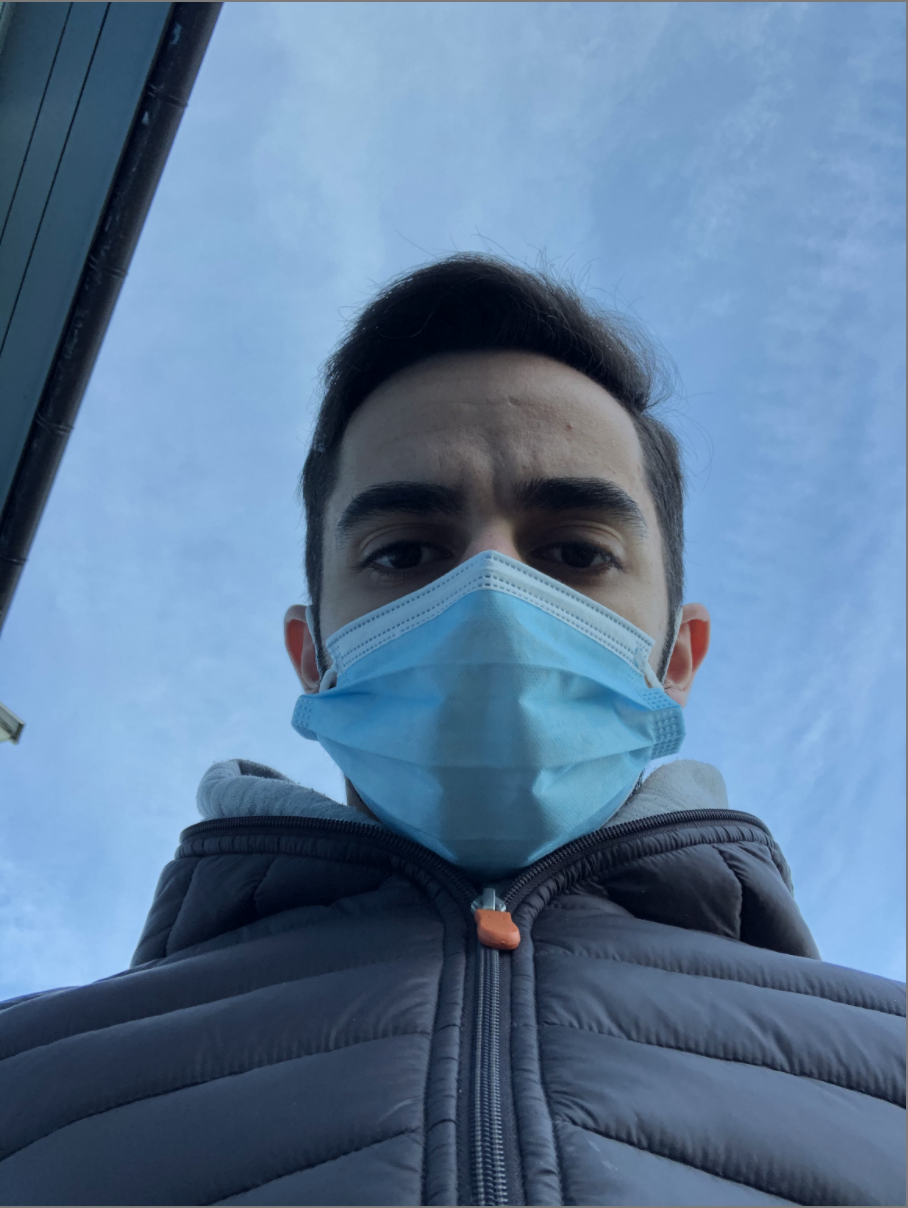
\includegraphics[scale = 0.18]{figures/1133.png}\hspace{1cm}}
    \subfloat[Mask below the nose]
        {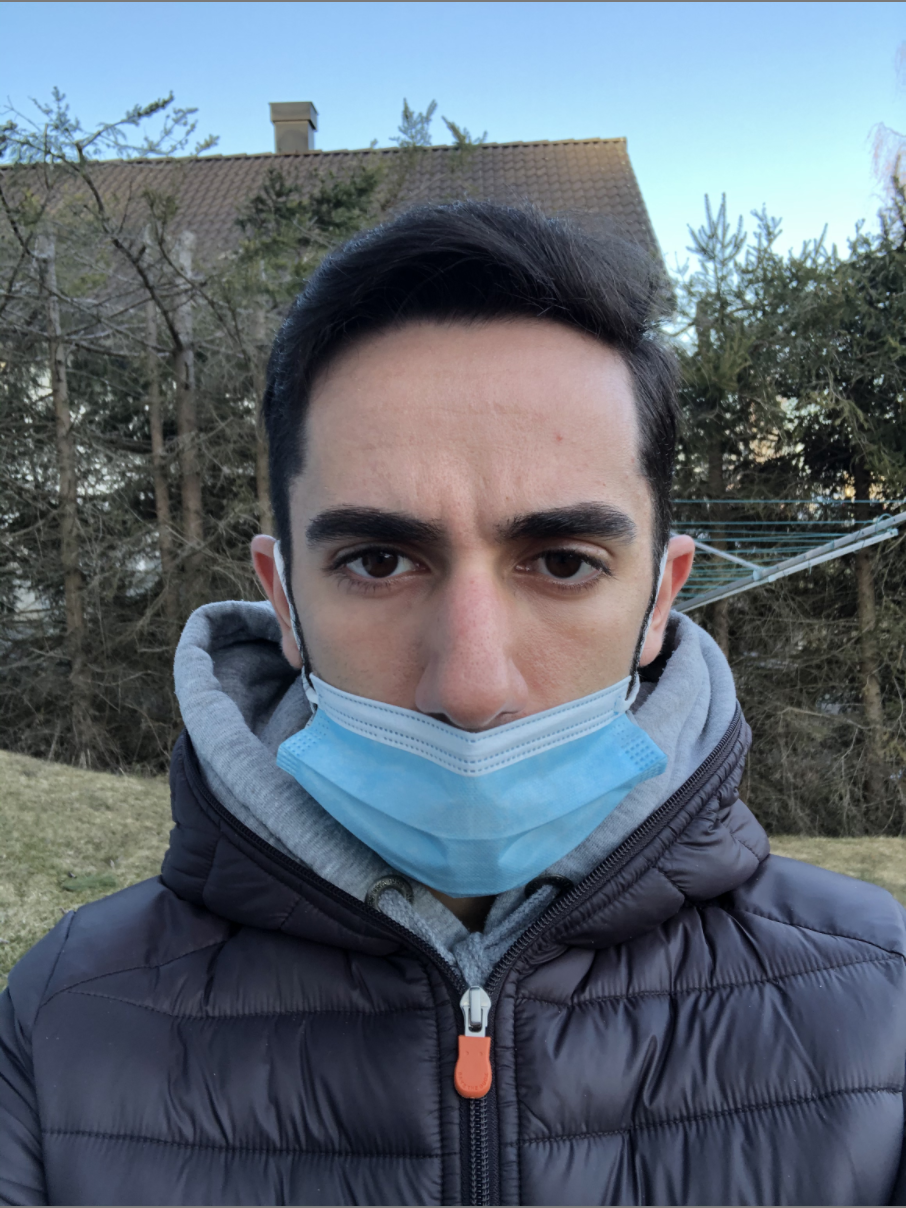
\includegraphics[scale = 0.18]{figures/940.png}\hspace{1cm}}
    \subfloat[Mask covering the chin]
        {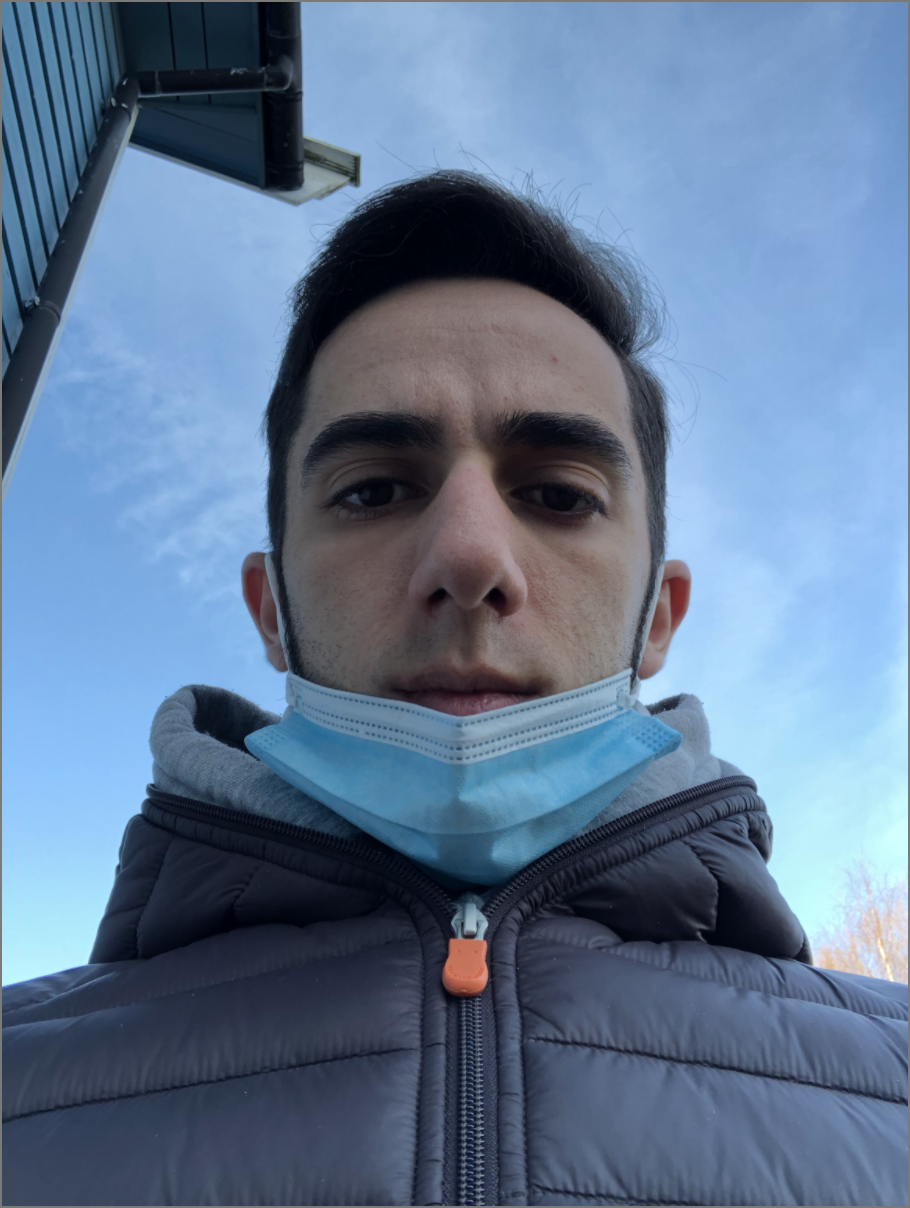
\includegraphics[scale = 0.18]{figures/1110.png}\hspace{1cm}}
    \subfloat[Mask below the chin]
        {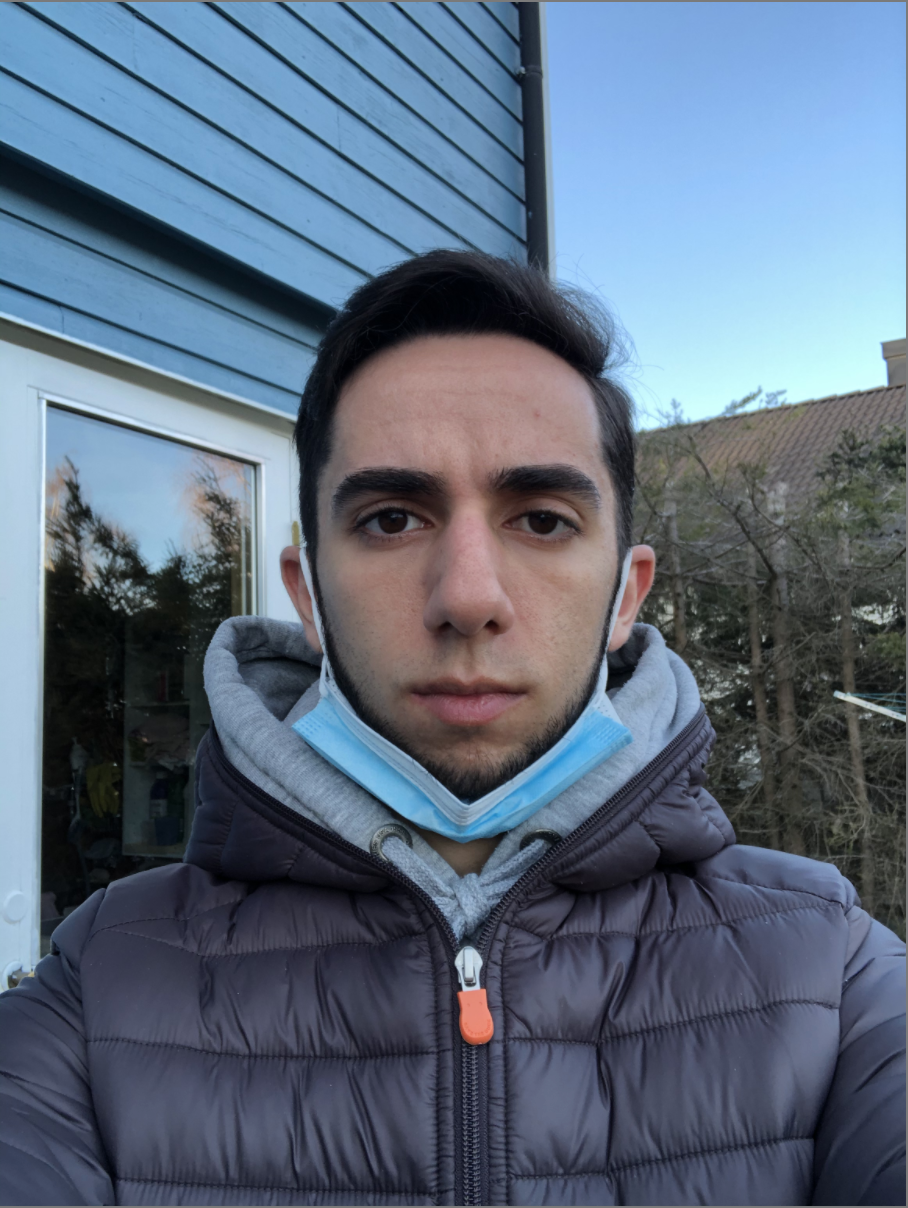
\includegraphics[scale = 0.18]{figures/1152.png}\hspace{1cm}}
    \caption{Different face masks usage.}
    \label{fig:masks}
\end{figure}
\subsection*{Camera Tilting}
The other important contribution to our dataset, was that we experimented with different camera tilts, also known as ``Dutch angle'' or ``oblique angles''. These types of images involves tilting the camera at an angle on its roll axis, which produces images where the viewpoint is similar to tilting one´s head to the side. Images like these create a form of disorientation because the camera has been rotated relative to the horizon of an image. This type of disorientation can be perceived by humans, but whether the FIQMs react differently towards these type of images is yet to be seen. For that reason, we wanted to look into dutch angle face images and see if the FIQMs produce significant different scores solely based on the camera tilt. 

\begin{figure}[h]
\centering
    \subfloat
        {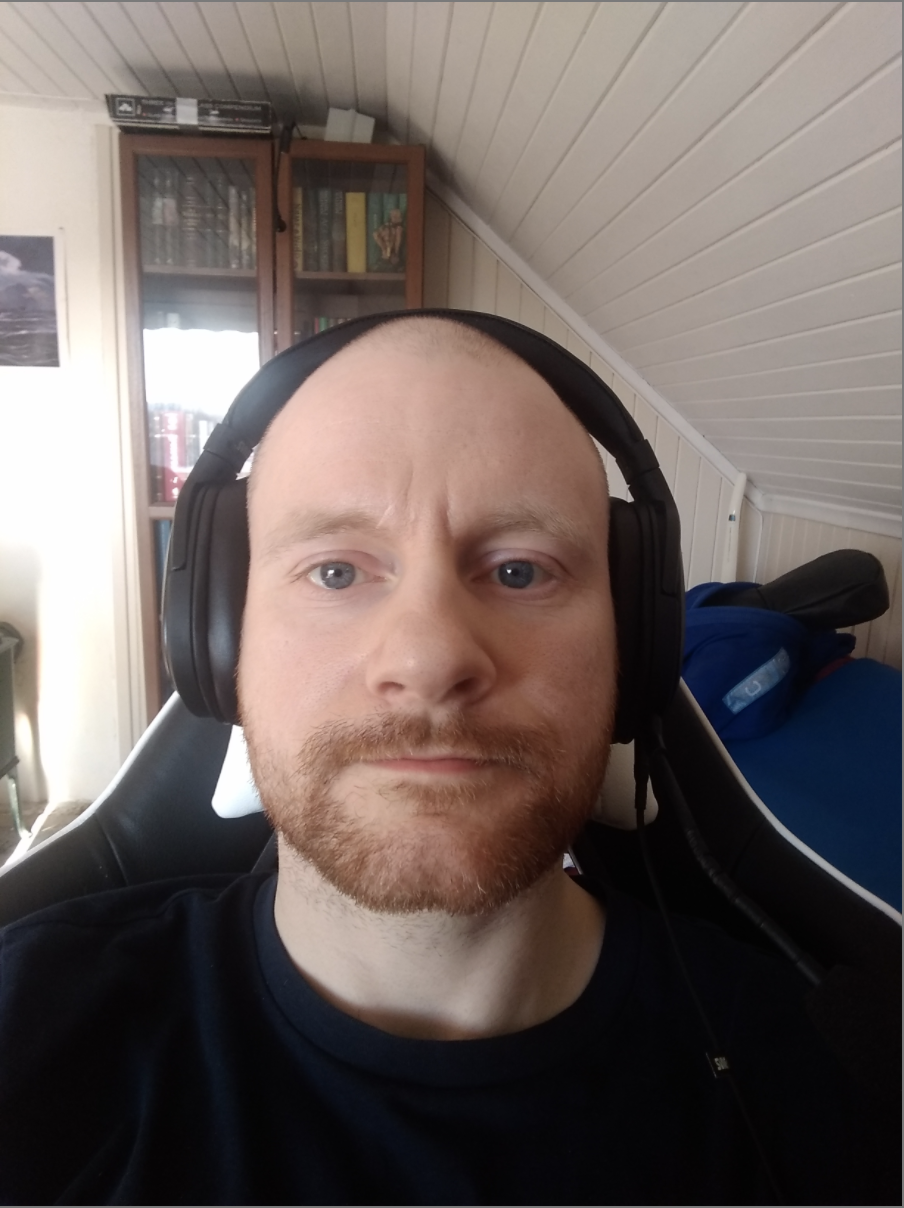
\includegraphics[scale = 0.2]{figures/0368.png}\hspace{1cm}}
    \subfloat
        {
\includegraphics[scale = 0.2]{figures/0367.png}\hspace{1cm}}
    \subfloat
        {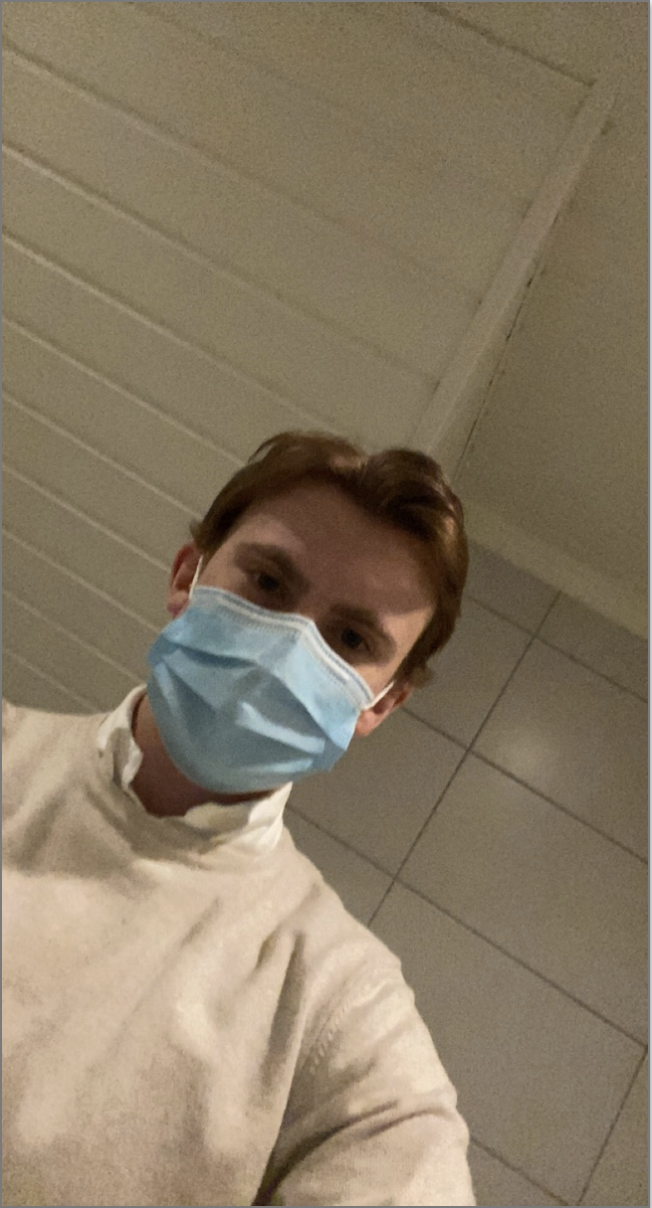
\includegraphics[scale = 0.2]{figures/0129.png}\hspace{1cm}}
    \subfloat
        {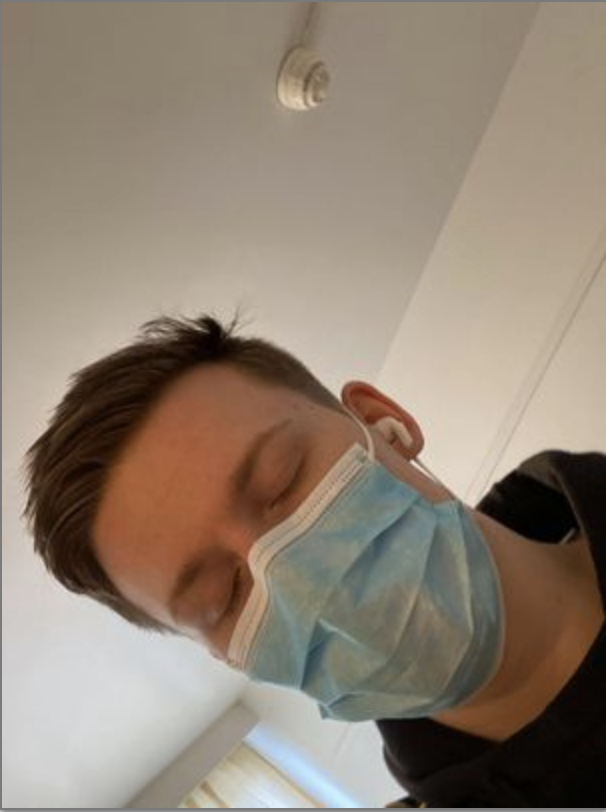
\includegraphics[scale = 0.295]{figures/0699.png}}
    \caption{Different camera angle shots.}
    \label{fig:tilt}
\end{figure}

As briefly mentioned in Section \ref{sec:delimit}, finding datasets that addressed and included face images taken from oblique angles were hard to come by. The closest datasets we came by, only included face images where the subjects had their heads tilted and not the camera which does not correspond to the same. Not only are the inclusion of the dutch angle face images quite new, but our dataset furthermore mixed these images with face masks, which created an even more distinct dataset. 

\subsection*{Labeling our Dataset}
The creation of our dataset would be lackluster had we not gathered the ground truth data for the images. However, gathering ground truth data for all 1172 images would require us to create a substantially large-scale subjective experiment. By the experience during the first one, as described in Section \ref{sec:ConductingSurvey}, this would take a lot of time and organizing. At that time, one month was left before the thesis was due and that would not be sufficient time. Since we had not yet planned to create our own dataset at the start of the semester, we felt a second subjective experiment of this size without proper planning would be destined to fail. Because of those reasons, we agreed to label only a small part of the dataset instead.  

Out of the 1172 images originally captured, 250 images were selected and used in our second subjective experiment. The images were selected equally between the members´ individual datasets to prevent that one member appeared more times than the others. Since 250 images cannot be equally split between four subjects, one member was represented two times less in the new dataset. Because these images were going to be used in the second subjective experiment we had to select images with different face image qualities. 

\section{Second Subjective Experiment}
\label{sec:secondse}
A key part we wanted to achieve with the second subjective experiment was to make it as straight forward and understandable as possible. One should not have to be trained once more in order to understand and perform the survey. Therefore, we designed the second survey as similar to our first one, given that no new participants were invited to participate. The ground truth data was collected by running the experiment with six people who were the bachelor team, our supervisor and the product owner. The key elements of the survey were: 
\begin{itemize}
    \item Randomizing the order of the images.
    \item Splitting it into two parts. 
    \item Using a category judgement.
\end{itemize}

The second experiment consisted of two parts. The first one included all 250 images from our selected dataset without splitting it into several connected survey sessions as we did in our first experiment. Since all participants already had knowledge about rating images, we did not feel the need to split it into multiple sessions. While splitting the survey would prevent participants from getting exhausted and bored, experience from our first survey showed that the average duration to finish a session with 100 images was shorter than expected. We had initially planned for a 100 image session to take up to 15 minutes, but feedback from our participants showed that most were finished after six to eight minutes. Based on those results, a survey with 250 images should not take longer than 25 minutes which is below the maximum limit of 30 minutes suggested by International Telecommunication Union \cite{methodologySubjective}. Although the survey was 2.5 times larger than the sessions of the first experiment, only people directly involved with the project were expected to participate. Creating several sessions felt like unnecessary overhead. 

%The main purpose of the second subjective experiment was to label our dataset of 250 images and test the FIQMs, but we felt it lacked a clear difference from the first subjective experiment, and we figured including distorted images would make the difference. The second part of the experiment was therefore made of 50 images, consisting of all subjects selected from the first dataset, but with distortions added to them. The point of the second part was to see whether the participants would evaluate the face image quality of an undistorted and distorted image the same, and whether the FIQMs followed that statement. If the participants valued the images the same and the FIQMs did not, then the FIQMs would not provide the right scores, given that the scores are based on human assessment.  

The main purpose of conducting the second subjective experiment was to label our dataset of 250 images. We would then run the dataset on the two FIQMs and compare results. We wanted to see how the two FIQMs would react if we gave them a dataset consisting of different aspects, like face masks and tilted camera. If the FIQMs' results differed drastically compared to the results from the subjective experiment, we could then conclude that the two FIQMs would only give accurate scores on a specific type of images. Our reason for conducting the second subjective experiment was therefore to test the two FIQMs further more, and also give the possibility for Mobai to test other FIQMs in the future, based on our subjective results. This was the first part of the second subjective experiment.

Even though our subjective experiment had new ways and aspects of testing the two FIQMs, we wanted to test them even further. The FIQMs ways of giving quality scores are based on how well you can see the face, explained in Chapter \ref{chap:FQA}, but the facial images' overall quality also matters. We wanted to see how the two FIQMs would react if we added distortions to them. Based on this, we decided to add different distortions to some images from our own dataset. Based on the results from the 250 images used in part one of our second subjective experiment, we selected 10 images from each quality category and added distortions to them. This gave us 50 images to add each distortion on. We chose to add four different distortions, giving us 200 distorted images. From there, we conducted another subjective experiment, identical in design from part one and with the same number of subjects. This is part two of the second subjective experiment. This subjective experiment consisted of the 200 distorted images, as well as the 50 original images selected from each quality category, giving us 250 images to rate.       

The type of distortions we added had to be reproducible, that way future research could add the same distortions and expect similar results. We added the following distortions:
%
\begin{itemize}
    \item Compression with Telegram: As our first compression, we used the cloud based messaging platform Telegram. The compression was done by messaging the images, resulting in change of the images' resolution and size.
    \item Compression with Adobe Photoshop: The other compression was done in Adobe Photoshop. All images were compressed with compression level one.
    \item Noise with Adobe Photoshop: The images were added with noise of seven percent. 
    \item Blur with Adobe Photoshop: The images were added a blur level of two. 
\end{itemize}
%


Having two parts in the second subjective experiment, both with a new dataset and added distortions, gives us a considerable amount of data to test the two FIQMs on. Based on part one and part two, we can compare the subjective results from both parts and see how the subject's scores differ with distortions added to the images. From there, we can test the two FIQMs results the same way and compare them directly with the subjective results. Ideally, both the FIQMs results and the subjective results should not differ in part one and part two as long as the distortions does not ruin how well you can see the face on the images.   
